


\tikzset{every picture/.style={line width=0.75pt}} %set default line width to 0.75pt        

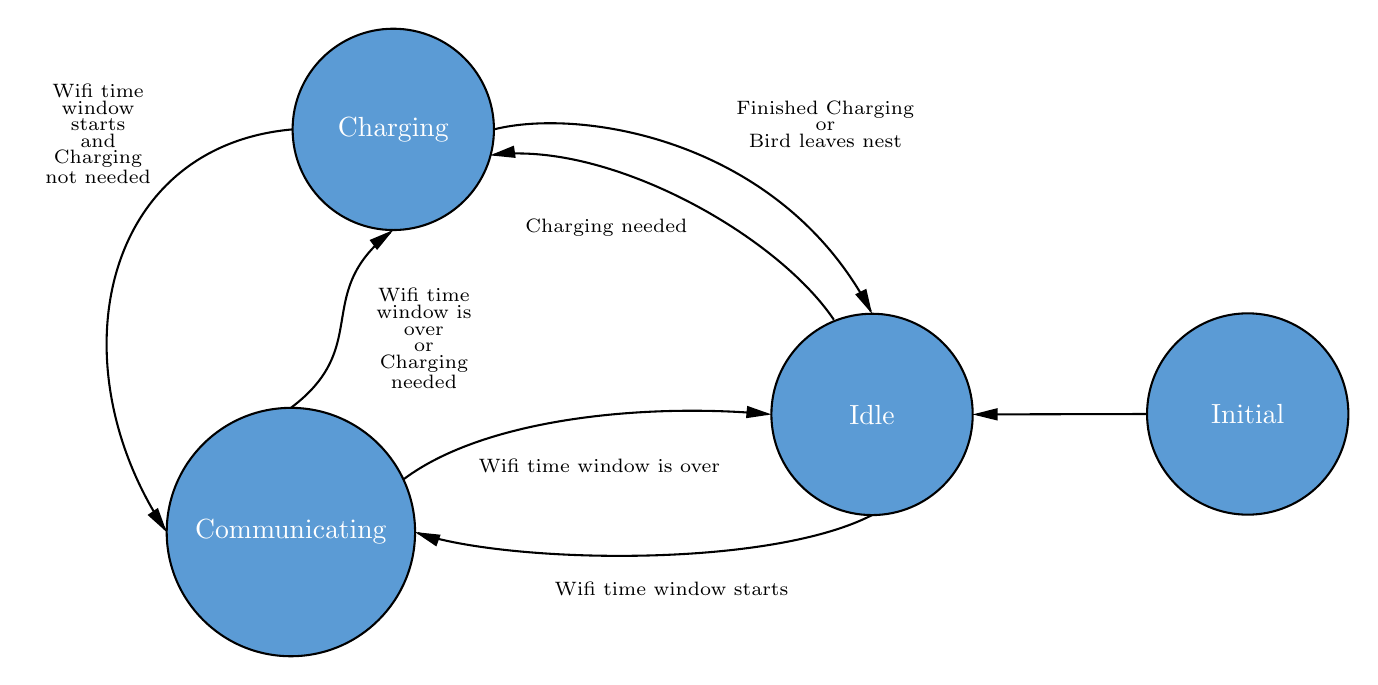
\begin{tikzpicture}[x=0.75pt,y=0.75pt,yscale=-1,xscale=1]
%uncomment if require: \path (0,372); %set diagram left start at 0, and has height of 372

%Shape: Circle [id:dp8124567583383704] 
\draw  [fill={rgb, 255:red, 91; green, 155; blue, 213 }  ,fill opacity=1 ] (145.83,94.5) .. controls (145.83,67.71) and (167.55,46) .. (194.33,46) .. controls (221.12,46) and (242.83,67.71) .. (242.83,94.5) .. controls (242.83,121.29) and (221.12,143) .. (194.33,143) .. controls (167.55,143) and (145.83,121.29) .. (145.83,94.5) -- cycle ;
%Shape: Circle [id:dp8370477309089557] 
\draw  [fill={rgb, 255:red, 91; green, 155; blue, 213 }  ,fill opacity=1 ] (85.16,288.51) .. controls (85.16,255.46) and (111.95,228.67) .. (144.99,228.67) .. controls (178.04,228.67) and (204.83,255.46) .. (204.83,288.51) .. controls (204.83,321.55) and (178.04,348.34) .. (144.99,348.34) .. controls (111.95,348.34) and (85.16,321.55) .. (85.16,288.51) -- cycle ;
%Shape: Circle [id:dp6759549796054376] 
\draw  [fill={rgb, 255:red, 91; green, 155; blue, 213 }  ,fill opacity=1 ] (376.5,231.83) .. controls (376.5,205.05) and (398.21,183.33) .. (425,183.33) .. controls (451.79,183.33) and (473.5,205.05) .. (473.5,231.83) .. controls (473.5,258.62) and (451.79,280.33) .. (425,280.33) .. controls (398.21,280.33) and (376.5,258.62) .. (376.5,231.83) -- cycle ;
%Shape: Circle [id:dp9540761941022562] 
\draw  [fill={rgb, 255:red, 91; green, 155; blue, 213 }  ,fill opacity=1 ] (557.5,231.63) .. controls (557.5,204.85) and (579.21,183.13) .. (606,183.13) .. controls (632.79,183.13) and (654.5,204.85) .. (654.5,231.63) .. controls (654.5,258.42) and (632.79,280.13) .. (606,280.13) .. controls (579.21,280.13) and (557.5,258.42) .. (557.5,231.63) -- cycle ;
%Curve Lines [id:da6761477491464263] 
\draw    (144.99,228.67) .. controls (160.53,217.01) and (165.41,206.01) .. (167.91,195.16) .. controls (171.76,178.41) and (169.95,162.02) .. (192.9,144.1) ;
\draw [shift={(194.33,143)}, rotate = 503.13] [fill={rgb, 255:red, 0; green, 0; blue, 0 }  ][line width=0.08]  [draw opacity=0] (12,-3) -- (0,0) -- (12,3) -- cycle    ;
%Curve Lines [id:da6639590384941882] 
\draw    (145.83,94.5) .. controls (53.46,102.57) and (31.62,207.95) .. (84.36,287.31) ;
\draw [shift={(85.16,288.51)}, rotate = 235.93] [fill={rgb, 255:red, 0; green, 0; blue, 0 }  ][line width=0.08]  [draw opacity=0] (12,-3) -- (0,0) -- (12,3) -- cycle    ;
%Curve Lines [id:da878040981951129] 
\draw    (242.83,94.5) .. controls (284.79,83.87) and (381.23,99.26) .. (424.35,182.08) ;
\draw [shift={(425,183.33)}, rotate = 242.98] [fill={rgb, 255:red, 0; green, 0; blue, 0 }  ][line width=0.08]  [draw opacity=0] (12,-3) -- (0,0) -- (12,3) -- cycle    ;
%Curve Lines [id:da9853831355446321] 
\draw    (406.6,186.21) .. controls (378.88,145.03) and (297.84,99.92) .. (242.66,106.79) ;
\draw [shift={(241,107.01)}, rotate = 351.75] [fill={rgb, 255:red, 0; green, 0; blue, 0 }  ][line width=0.08]  [draw opacity=0] (12,-3) -- (0,0) -- (12,3) -- cycle    ;
%Curve Lines [id:da5001005141054524] 
\draw    (199.4,263.01) .. controls (239,233.31) and (316.92,226.4) .. (374.75,231.67) ;
\draw [shift={(376.5,231.83)}, rotate = 185.48] [fill={rgb, 255:red, 0; green, 0; blue, 0 }  ][line width=0.08]  [draw opacity=0] (12,-3) -- (0,0) -- (12,3) -- cycle    ;
%Curve Lines [id:da7814999567286496] 
\draw    (425,280.33) .. controls (374.02,306.5) and (248.35,303.48) .. (206.09,288.95) ;
\draw [shift={(204.83,288.51)}, rotate = 380] [fill={rgb, 255:red, 0; green, 0; blue, 0 }  ][line width=0.08]  [draw opacity=0] (12,-3) -- (0,0) -- (12,3) -- cycle    ;
%Straight Lines [id:da16727934758117113] 
\draw    (557.5,231.63) -- (475.5,231.83) ;
\draw [shift={(473.5,231.83)}, rotate = 359.86] [fill={rgb, 255:red, 0; green, 0; blue, 0 }  ][line width=0.08]  [draw opacity=0] (12,-3) -- (0,0) -- (12,3) -- cycle    ;

% Text Node
\draw (194.33,94.5) node   [align=left] {\textcolor[rgb]{1,1,1}{Charging}};
% Text Node
\draw (144.99,288.51) node   [align=left] {\textcolor[rgb]{1,1,1}{Communicating}};
% Text Node
\draw (425,231.83) node   [align=left] {\textcolor[rgb]{1,1,1}{Idle}};
% Text Node
\draw (606,231.63) node   [align=left] {\textcolor[rgb]{1,1,1}{Initial}};
% Text Node
\draw (402.5,91.91) node  [font=\tiny] [align=left] {\begin{minipage}[lt]{79.56pt}\setlength\topsep{0pt}
\begin{center}
{\scriptsize Finished Charging}\\{\scriptsize or}\\{\scriptsize Bird leaves nest}
\end{center}

\end{minipage}};
% Text Node
\draw (297,141.66) node  [font=\tiny] [align=left] {\begin{minipage}[lt]{76.16pt}\setlength\topsep{0pt}
\begin{center}
{\scriptsize Charging needed}
\end{center}

\end{minipage}};
% Text Node
\draw (293.6,256.76) node  [font=\tiny] [align=left] {\begin{minipage}[lt]{117.5pt}\setlength\topsep{0pt}
\begin{center}
{\scriptsize Wifi time window is over}
\end{center}

\end{minipage}};
% Text Node
\draw (328.4,316.06) node  [font=\tiny] [align=left] {\begin{minipage}[lt]{105.54pt}\setlength\topsep{0pt}
\begin{center}
{\scriptsize Wifi time window starts}
\end{center}

\end{minipage}};
% Text Node
\draw (52.1,96.67) node [font=\tiny] [align=left] {\begin{minipage}[lt]{44.21pt}\setlength\topsep{0pt}
\begin{center}
{\scriptsize Wifi time window starts}\\{\scriptsize and}\\{\scriptsize Charging not needed}
\end{center}

\end{minipage}};
% Text Node
\draw (209.09,195.18) node  [font=\tiny] [align=left] {\begin{minipage}[lt]{46.25pt}\setlength\topsep{0pt}
\begin{center}
{\scriptsize Wifi time window is over}\\{\scriptsize or}\\{\scriptsize Charging needed}
\end{center}

\end{minipage}};


\end{tikzpicture}